\section{Reimplementation Strategy}
\label{sec:remplementation}

The main purpose of my implementation work was to be able to code by myself some of the core ideas of the ADOP differentiable point based neural renderer.
I decided to code everything from scratch knowing since the start that I would at no point be able to fully reproduce the results from the authors but I learnt a large amount of things by doing so.
\begin{itemize}
    \item I used BlenderProc \cite{Denninger2023} to script and generate multiple synthetic scenes from the samples used in the NerF paper. All camera positions are known and share the same referential as my pytorch point renderer.
    \item A perfect point cloud is sampled at random from the mesh (through the .obj file).
    \item A pytorch function allows to project the points onto the image plane and includes soft depth test and normal culling.
\end{itemize}

Each element has been carefully tested by mostly visual tests.






\subsection{Generating synthetic calibrated scenes}
\label{sec:synthetic_calibrated_scenes}
In order to avoid dealing with large real scenes with millions of points and having to deal with heavy COLMAP processing, I decided to use a recent library named BlenderProc  \cite{Denninger2023} which simplifies the use of Blender as it allows running renders in the background (launched through terminal without the need of a graphical user interface).

It is first possible to generate a set of viewpoints configurations to orbit around the scene. It is also possible to generate an environment map (e.g. a skybox). We render with the background transparency option so the rendering results is a RGB PNG. 
% 1532.9s for 60 views of the \texttt{material balls}.

Rendering is peformed using GPU and requires 25 seconds per view with a resolution 640x480 for the \texttt{material balls}. scene on a laptop Nvidia T500.

\begin{figure}[H]
    \centering
    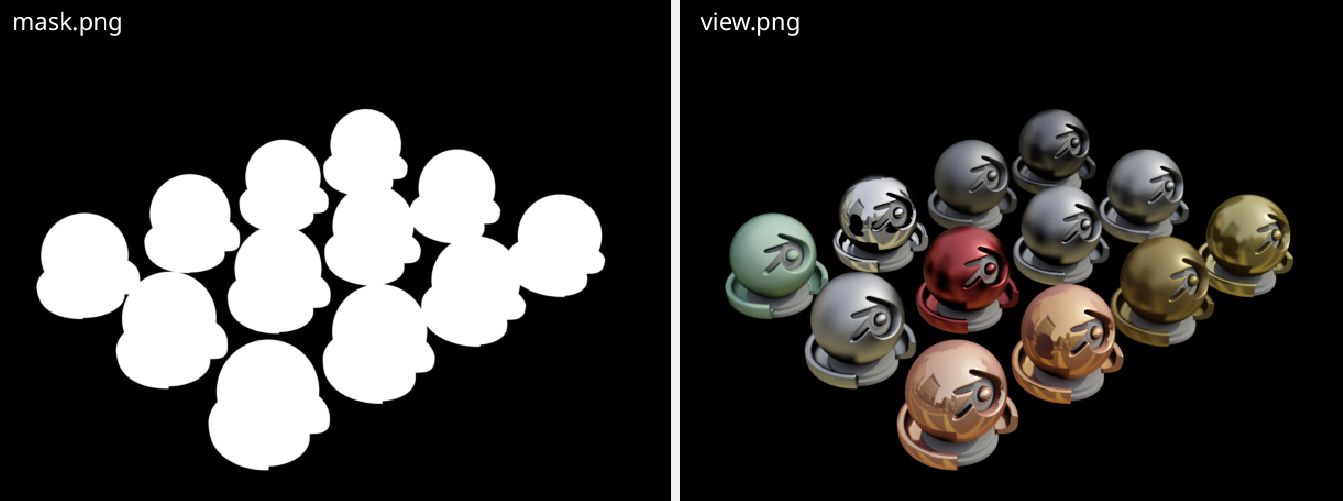
\includegraphics[width=0.5\textwidth]{figures/blenderproc_renders.png}
    \caption{Mask and RGB render BlenderProc renders with an environment map.}
    \label{fig:blenderproc_renders}
\end{figure}


% 27 minutes are needed to generate 64 viewpoints
The environment map does not appear as a backround (although it is possible in the current code) as it would allow to simplify and remove one of the extra components of the ADOP paper (e.g. it allows rendering the point cloud without using the neural environment map trick).

We parameterize camera orientation using 3 Euler Angles (yaw pitch roll) and 3 positions. When we project a point onto the image plane, we build the extrinsic camera matrix from the. We use a pinhole camera model.